%% TCC - Monografia
%% Ci\^{e}ncia da Computa\c{c}\~{a}o - LCMAT - CCT - UENF, 2018
%% 

\chapter{Metodologia}\label{cap3}

O propósito deste trabalho é realizar um estudo descritivo sobre as arquiteturas em camadas e microsserviços. A abordagem da pesquisa será qualitativa de caráter exploratório, pois iremos focar no caráter subjetivo do objeto analisado. 

O método que será utilizado para a realização deste trabalho é o qualitativo, com a finalidade de implementar e analisar as arquiteturas, assim poderemos fazer um estudo descritivo sobre as duas arquiteturas ilustradas nesta pesquisa. Em relação ao caráter exploratório serão aplicados alguns problemas na arquitetura e analisaremos o seu comportamento.

Serão obtidos os dados necessários para essa pesquisa através das pesquisas bibliográficas, da implementação e da observação comportamental do software diante de alguns problemas que serão colocados em um ambiente controlado. Com toda essa abordagem, poderemos descrever os resultados obtidos.

A pesquisa seguirá algumas fases, que serão resumidas na sequência: 
\begin{enumerate}
    \item Revisão bibliográfica
    \item Criação do fluxo das duas arquiteturas estudadas.
    \item Implementação da arquitetura em camadas:
    \begin{itemize}
        \item Coleta de dados durante a implementação
        \item Realização de experimentos
        \item Recuperação de informação
    \end{itemize}
    
    \item  Implementação da arquitetura baseada em microsserviços:
        \begin{itemize}
        \item Coleta de dados durante a implementação
        \item Realização de experimentos
        \item Recuperação de informação
    \end{itemize}
    \item Conclusão das informações em relação à: 
    \begin{itemize}
        \item Escalabilidade, 
        \item Manutenibilidade, 
        \item Implementação computacional, assim como
        \item Vantagens e Desvantagens.
    \end{itemize}
    
\end{enumerate}

Na Figura \ref{fig:flow-metodologia} é possível observar o fluxograma da metodologia que acabamos de apresentar e que faz parte deste trabalho de pesquisa.

\begin{figure}[htbp]
    \hypertarget{arquitetura-camadas2}{%
        \caption{ Fluxograma da metodologia utilizada neste trabalho}
        \begin{center}
          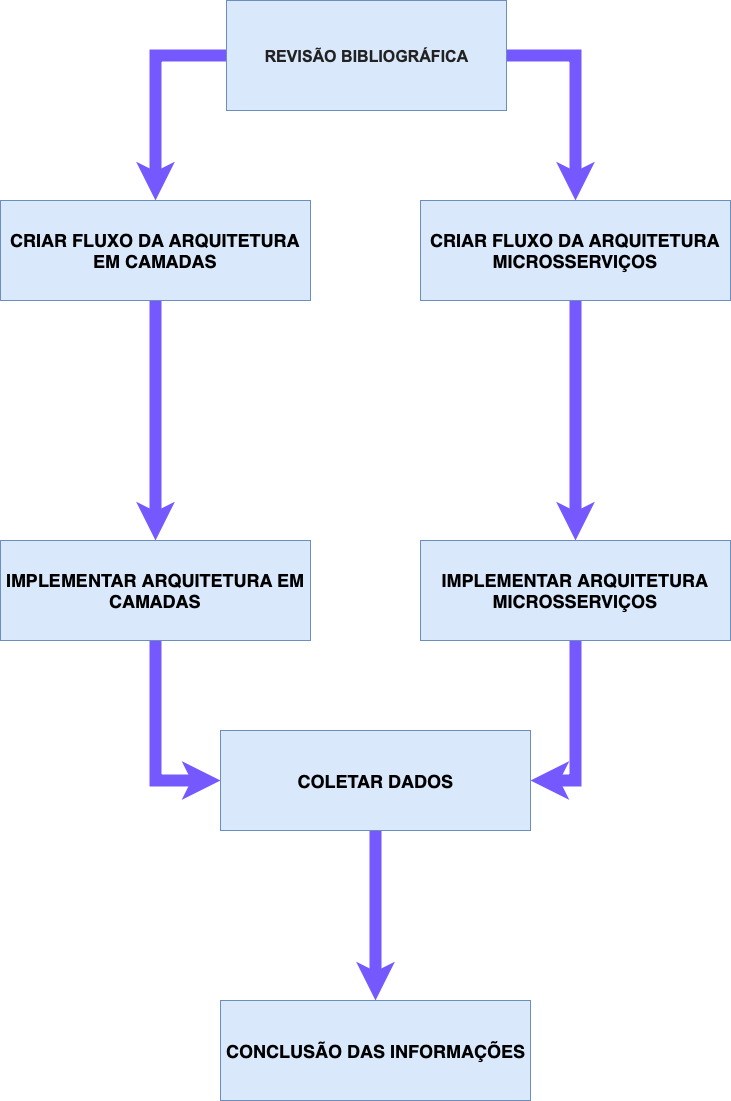
\includegraphics[width=10cm]{Monografia-FormatoLatex/Imagens/flow-metodologia.png}
        \end{center}
    }
    \legend{Fonte: Imagem feita pelo autor no site \url{draw.io}}
    \label{fig:flow-metodologia}
\end{figure}

\section{Revisão bibliográfica}
Durante essa fase, realizada no capítulo \ref{cap2}, a pesquisa buscou reunir as definições de diversos autores sobre as arquiteturas, tanto a baseada em camadas, quanto a baseada em microsserviços. Durante essa fase é importante entender o fluxo comportamental de ambas, abordagens relacionadas, informações sobre sistemas distribuídos. De modo geral nessa fase o mais importante é entender sobre as arquiteturas e porque utilizar uma ou outra.

\section{Fase 2 - Criação do fluxo das arquiteturas }

É importante durante a criação de um fluxograma para buscar a melhor tecnologias para esse tipo de projeto, para no processo de implementação utilizar a ferramenta que resolve da melhor forma aquele problema e levar em consideração também a experiência da equipe ou desenvolvedor que irá construir o sistema. O fluxo deve ser feito descrevendo a comunicação entre cada sistema ou tecnologia.

Durante essa fase faremos um levantamento de requisitos para as tecnologias que melhor se adequará a arquitetura em camadas e a expertise do desenvolvedor. Com a definição dessa tecnologia poderemos criar um fluxograma e de forma visual mostrar a comunicação entre as camadas, assim facilitaremos a visualização por parte de outros membros da equipe ou mesmo de uma pessoa leiga que necessite entender de forma clara e simples.

Com todas as ferramentas e tecnologias definidas, poderemos desenhar o fluxo da arquitetura em camadas e o fluxo da arquitetura baseada em Microsserviços.

\section{Fase 3 - Implementação da arquitetura em camadas e arquitetura baseada em Microsserviços}

Durante a fase de implementação, o objetivo é realmente desenvolver um sistema seguindo o fluxograma da fase 2. A implementação será feita pensando em um ambiente real, assim poderemos simular um ambiente de produção, com as tecnologias e ferramentas do dia a dia de trabalho de uma empresa.

\section{Fase 4 - Coleta de dados}

Durante a fase de implementação e também após a mesma, será feita a coleta de dados, assim será feito os devidos experimentos e transformando os dados em informações para a geração de uma conclusão sobre cada arquitetura.

\section{Fase 6 - Conclusão das informações}

Com os dados já transformados em informações, o trabalho poderá ter uma conclusão real sobre a escalabilidade, manutenibilidade, a implementação de cada arquitetura e suas vantagens e desvantagens e outros insights.